\graphicspath{{06-Tracker/Figures/}}

\section{Trackers}
\label{Sect:Tracker}

\subsection{Introduction}
MICE is equipped with two identical, high precision scintillating-fibre trackers, described in~\cite{Ellis:2010bb}. Each tracker is placed in a superconducting solenoid designed to provide a uniform magnetic field over the tracking volume. One tracker, TKU, is upstream of the cooling cell, the other, TKD, is downstream, the mirror image of TKU as in Fig.~\ref{fig:BL}.

The trackers are 110\,cm in length and 30\,cm in diameter (see Fig.~\ref{Figure:FullTracker}). There are five stations per tracker (labelled 1 to 5, with station 1 being closest to the cooling cell) held in position using a carbon-fibre space-frame. The stations sit at varying separations in $z$ (beam axis) of 20--35\,cm: this ensures that the azimuthal rotation of track position from one station to the next differs, difference being important in resolving ambiguities at the pattern-recognition stage. Each tracker is instrumented with an internal LED calibration system for calibration and four 3-axis Hall probes to monitor the field.

\begin{figure}[ht]
\begin{center}
\includegraphics[width=0.6\textwidth,keepaspectratio=true,]{FullTracker.png}
\end{center}
\caption{Photograph of one of the MICE Trackers, showing the five stations and the three doublet planes of scintillating fibres, each plane at 120$^\circ$ angles to the next (the central fibres of plane can be seen as darker lines traversing the station). Bundles of seven 350$\mu m$ fibres are grouped together, to be read out by 1\,mm scintillating fibre light guides.}
\label{Figure:FullTracker}
\end{figure}

The tracker stations consists of three doublet layers of 350$\mu m$ scintillating fibres, these layers are arranged such that each is at an angle of 120$^\circ$ to the next. This arrangement ensures that there are no inactive regions between adjacent fibres. Bundles of seven fibres are grouped into a single readout channel (this reduces the number of readout channels, while maintaining position resolution). The trackers have a spatial resolution per doublet layer of 470$\mu m$ and an expected light yield of $\sim$ 10 photo-electrons.

The light from the seven scintillating fibres passes into a single clear fibre, which takes it to a visible light photon counter (VLPC) which operate at 9\,k. The signals from the VLPCs are digitised using electronics developed by the D0 collaboration~\cite{Abazov:2005pn}.


\subsection{Performance and Reconstruction}

Each of the 15 tracker planes (three per station and five stations) consist of 214 channels, labelled 0--213, likewise each plane is assigned an integer plane number 0--2. Particle signals are recorded by the tracker electronics and calibrated channel by channel then converted into signal NPE. This information is then used to form a digit and is the first step in tracker reconstruction.
Digit profiles are useful in identifying and rectifying or removing hot or dead channels in the planes and ensuring the accuracy of calibration.  Smooth centrally peaked spectra are expected in a plane with no dead channels and minimal electronics noise, but this is not an essential requirement since it is the combination of two or three planes which go to make a point in the track and so there is redundancy built in. Hence a significant proportion of individual channels can be lost without a knock on drop in efficiency. 
The clustering algorithm loops over every combination of pairs of digits in a single event and combines any that occur in neighbouring channels. In the case of a multi-digit cluster, the unweighted average channel value is used to define the plane coordinate and the NPE is summed.

%\begin{figure}[!ht]
%\begin{center}
%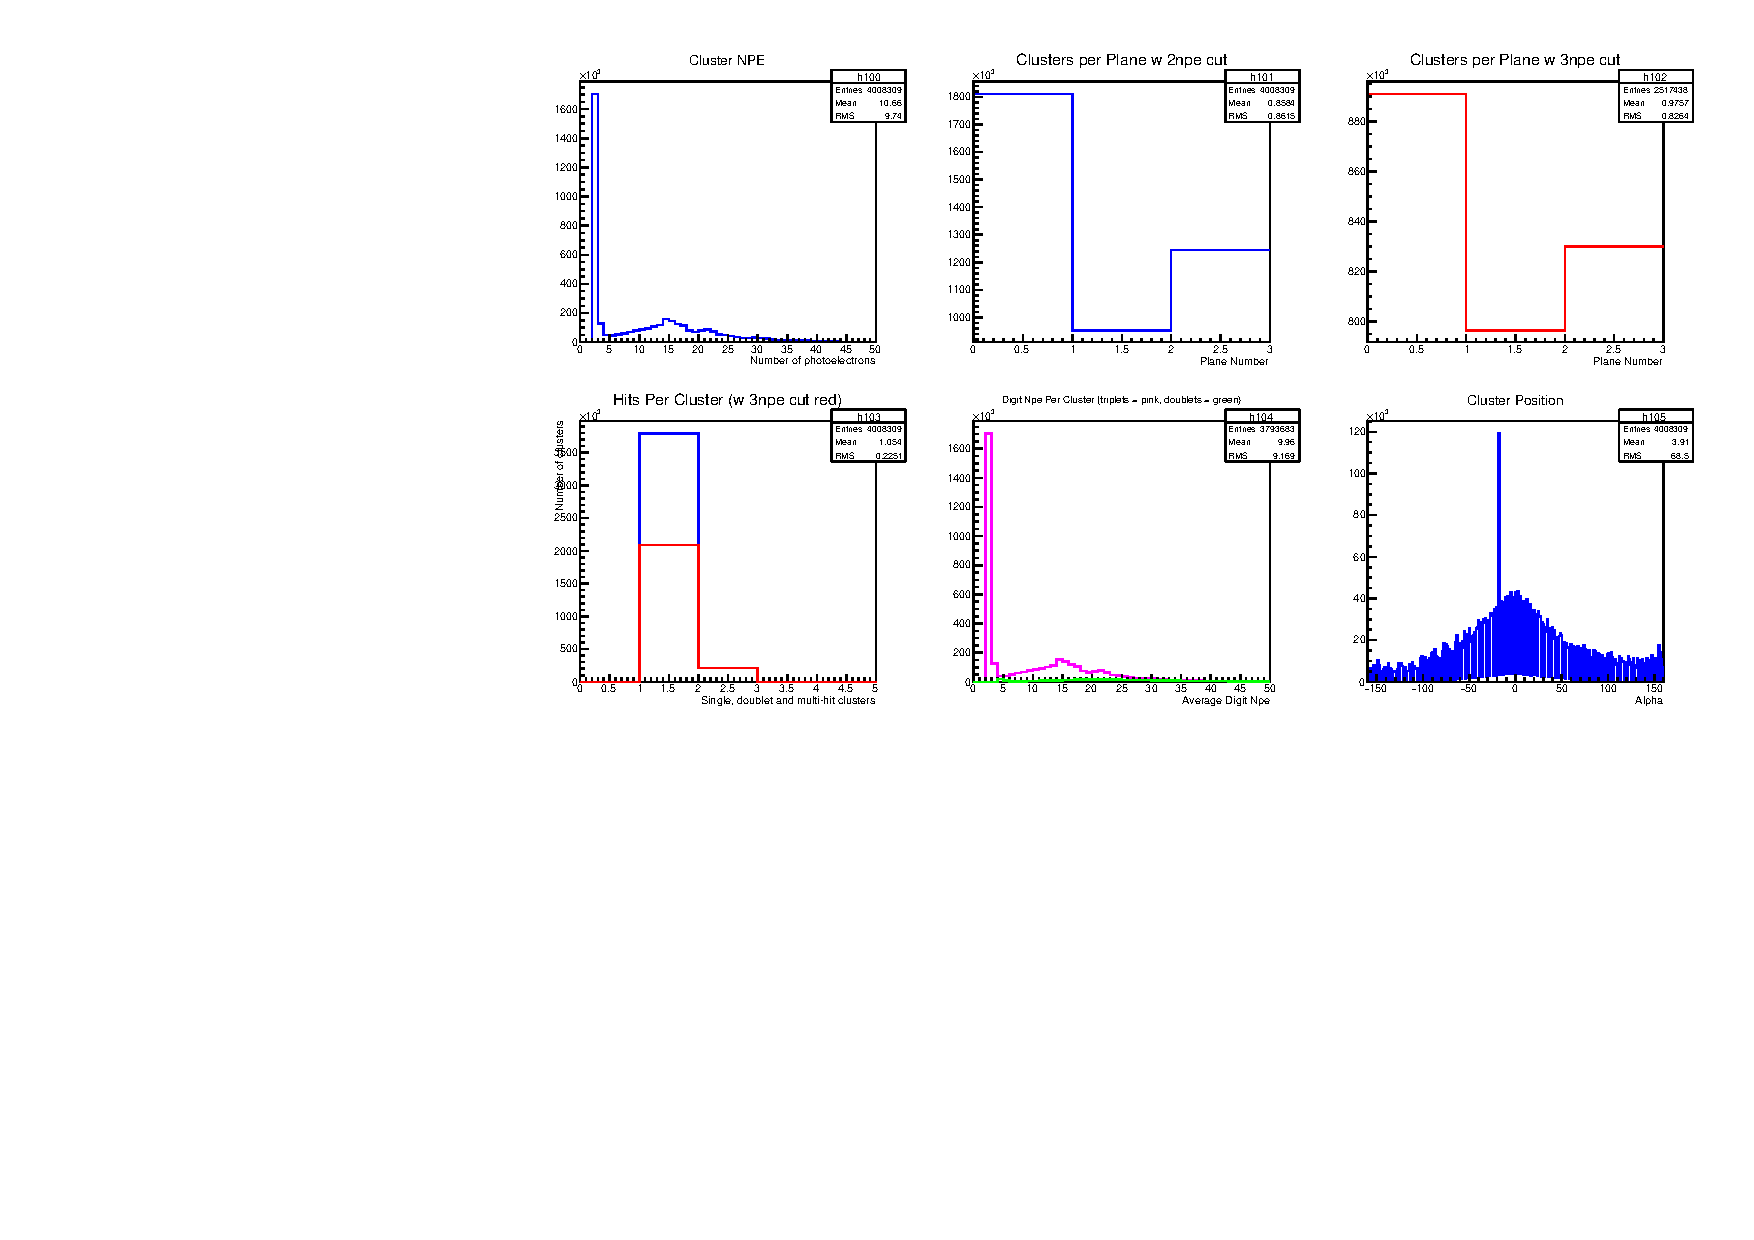
\includegraphics[width=0.9\textwidth,keepaspectratio=true,]{Clusters.pdf}
%\end{center}
%\caption{Cluster}
%\label{Figure:Clusters}
\%end{figure}

For each station the constituent planes are searched for clusters that can be used to form a spacepoint.
Spacepoints are constructed from clusters from all three planes (a triplet spacepoint) or from any two out of the three planes (a doublet spacepoint).

%\begin{figure}[!ht]
%\begin{center}
%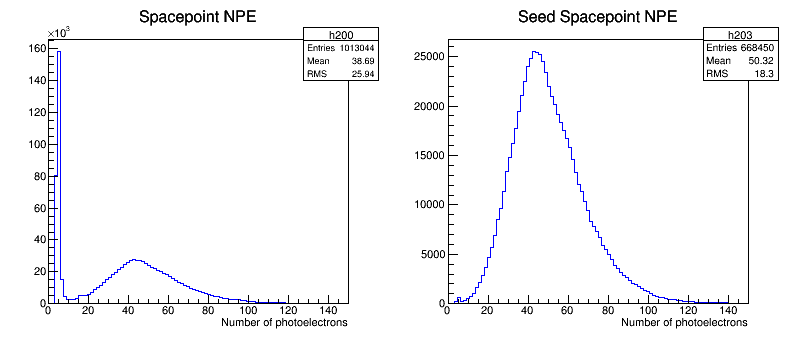
\includegraphics[width=0.75\textwidth,keepaspectratio=true,]{SPSeeds10314.png}
%\end{center}
%\caption{(Left) the NPE of each spacepoint in the US and DS trackers combined. (Right) only the NPE of those spacepoints which go on to make tracks in the US and DS %trackers combined are shown.}
%\label{Figure:SPSeeds_10314}
%\end{figure}

\subsubsection{Noise}
%Noise at electronics level discussion, 1/2 page, and Noise from data, 1/2 page.
The scintillating fibre trackers operate by registering digits above a given NPE threshold within each fibre plane. Fibres are collected into channels as ganged bundles of 7 for each channel, with digits are registered per channel instead of per fibre. From a coincidence of digit events in 2 or 3 oblique fibres (fibres in differing planes), a spacepoint is reconstructed, from which track reconstruction can occur. We consider noise in the tracker to be those digits registered not from the passage of a beam particle, but instead from other sources, for instance, dark current from thermal electron emission in the PMTs. To isolate noise from signal during beam-on data collection, a strict cut can be made requiring that only events with one fitted track and 5 spacepoints per tracker are selected, with all 5 spacepoints included in the fitted track. All digits corresponding to the track are then removed from the total set of digits for that event, and the remainder are considered noise digits. An in-situ approximation of active channels for the current data-taking period is made, assuming all channels without at least one registered digit in the selected data-taking run are inactive. The average noise rate per channel per event is then calculated as the total number of event digits above the considered NPE threshold in each tracker, divided by both the active channel number and the number of events satisfying the above selection criteria. This gives a value of 0.18\% upstream and 0.06\% downstream for events above 2~NPE. 

\subsubsection{Track Finding Efficiency}
\label{trackers:performance:efficiency}
%Track selection/Kalman, efficiency (from all data runs plotted by pt and if all equal just 10mm can be shown) resolution (from MC), reference MAUS and Tracker SW paper, 1 page, Chris H.
Data were analysed in order to determine the track and spacepoint finding efficiency of the detectors during running conditions. A time-of-flight cut was used to ensure that each measured track had a time-of-flight consistent with a muon throughout the entire experimental apparatus. A hit was therefore required in each of the TOF1 and TOF2 detectors, which ensured that the particle must have been successfully transmitted through the cooling channel, crossing both tracking detectors. These requirements ensure that there is a better then 99.9\% probability that a particle will have traversed a tracking detector. The number of events missing a track is therefore measured and used to estimate the efficiency of the detector.

The results of the efficiency analysis are tabulated in table~\ref{Table:tracker_efficiency_results} for a range of momentum and nominal emittances. A track-finding efficiency of 98.70\% is reported for the upstream tracker and 98.93\% for the downstream tracker, averaged over field and beam conditions. Additionally, assuming a track is found, the probability of successfully finding each spacepoint is summarized in table~\ref{Table:tracker_spacepoint_efficiency_results}. The overall efficiency of both trackers is sufficient to not present any significant systematic uncertainties in the analysis, however it is lower than the ideal expectation, 99.9\% efficiency, due to the presence of dead channels, an unavoidable feature of the construction process.

\begin{table}[ht]
	\centering
%    \begin{tabular}{c | c | c | c | c}
%    	\multirow{2}{*}{Run Number} & \multicolumn{2}{c}{Upstream} & \multicolumn{2}{c}{Downstream} \\
%                   &   No. Events  & Tracks Found &  No. Events & Tracks Found \\
%        09768 & 637 & 99.53\% & 1289 & 96.28\% \\
%        09952 & 5432 & 98.62\% & 5084 & 99.37\% \\
%        09959 & 3295 & 98.79\% & 3781 & 99.42\% \\
%        09964 & 892 & 98.09\% & 850 & 99.29\% \\
%        10510 & 3676 & 99.54\% & 2911 & 99.48\% 
%    \end{tabular}
    \begin{tabular}{c | c | c | c | c}
%      	\multirow{2}{*}{Momentum} & Nominal & \multirow{2}{*}{No. Events} & Upstream & Downstream \\
%                   & Emittance &  & Tracks Found & Tracks Found \\ \hline
        Momentum & Nominal Emittance & No. Events & Upstream Tracks Found & Downstream Tracks Found \\ \hline
        200 MeV/c & 6mm  & 221879 & 99.42\% & 96.07\% \\ %H25c 
        200 MeV/c & 3mm  & 215229 & 98.38\% & 99.19\% \\ %H36aa
        %\multirow{3}{*}{140 MeV/c} & 3mm & 215229 & 98.38\% & 99.19\% \\ %H36aa
        140 MeV/c & 6mm  & 180283 & 98.37\% & 99.16\% \\ %H36c
        140 MeV/c & 10mm & 130859 & 98.47\% & 98.93\% \\ \hline \hline %H36d
        \multicolumn{2}{c |}{Averaged} & 748250 & 98.70\% & 98.21\%
    \end{tabular}
    \caption{\label{Table:tracker_efficiency_results}The track finding efficiency for the upstream and downstream trackers for 140~MeV/c and 200~MeV/c beams, and for 3, 6 and 10~mm nominal emittances.}
\end{table}

\begin{table}[ht]
	\centering
    \begin{tabular}{c | c | c | c | c}
%   	\multirow{2}{*}{Momentum} & Nominal & \multirow{2}{*}{No. Events} & Upstream & Downstream \\
%                   & Emittance &  & Spacepoints Found & Spacepoints Found \\ \hline
       Momentum & Nominal Emittance & No. Events & Upstream Spacepoints Found & Downstream Spacepoints Found \\ \hline
        200 MeV/c & 6mm  & 221879 & 99.41\% & 94.63\% \\ %H25c 
%        \multirow{3}{*}{140 MeV/c} & 3mm & 215229 & 98.04\% & 97.41\% \\ %H36aa
        200 MeV/c & 3mm  & 215229 & 98.04\% & 97.41\% \\ %H36aa
        140 MeV/c & 6mm  & 180283 & 97.99\% & 99.16\% \\ %H36c
        140 MeV/c & 10mm & 130859 & 98.07\% & 97.44\% \\ \hline \hline %H36d
        \multicolumn{2}{c |}{Averaged} & 748250 & 98.44\% & 97.01\%
    \end{tabular}
    \caption{\label{Table:tracker_spacepoint_efficiency_results}The spacepoint finding efficiency, assuming the presence of a track, for the upstream and downstream trackers for 140~MeV/c and 200~MeV/c beams, and for 3, 6 and 10~mm nominal emittances.}
\end{table}

\subsubsection{Track Fit Predicted Performance}

Monte Carlo simulation used with realistic field and beam conditions in order to estimate the reconstruction performance. Run number 09964 was used (140~MeV/c, 10~mm nominal emittance), representing a typical data set used for the study of emittance evolution.
Results are presented in Fig.~\ref{trackers:performance:resolutions:up} for the upstream tracker and Fig.~\ref{trackers:performance:resolutions:down} for the downstream tracker.

\begin{figure}[ht]
	\centering
    \begin{tabular}{cc}
	    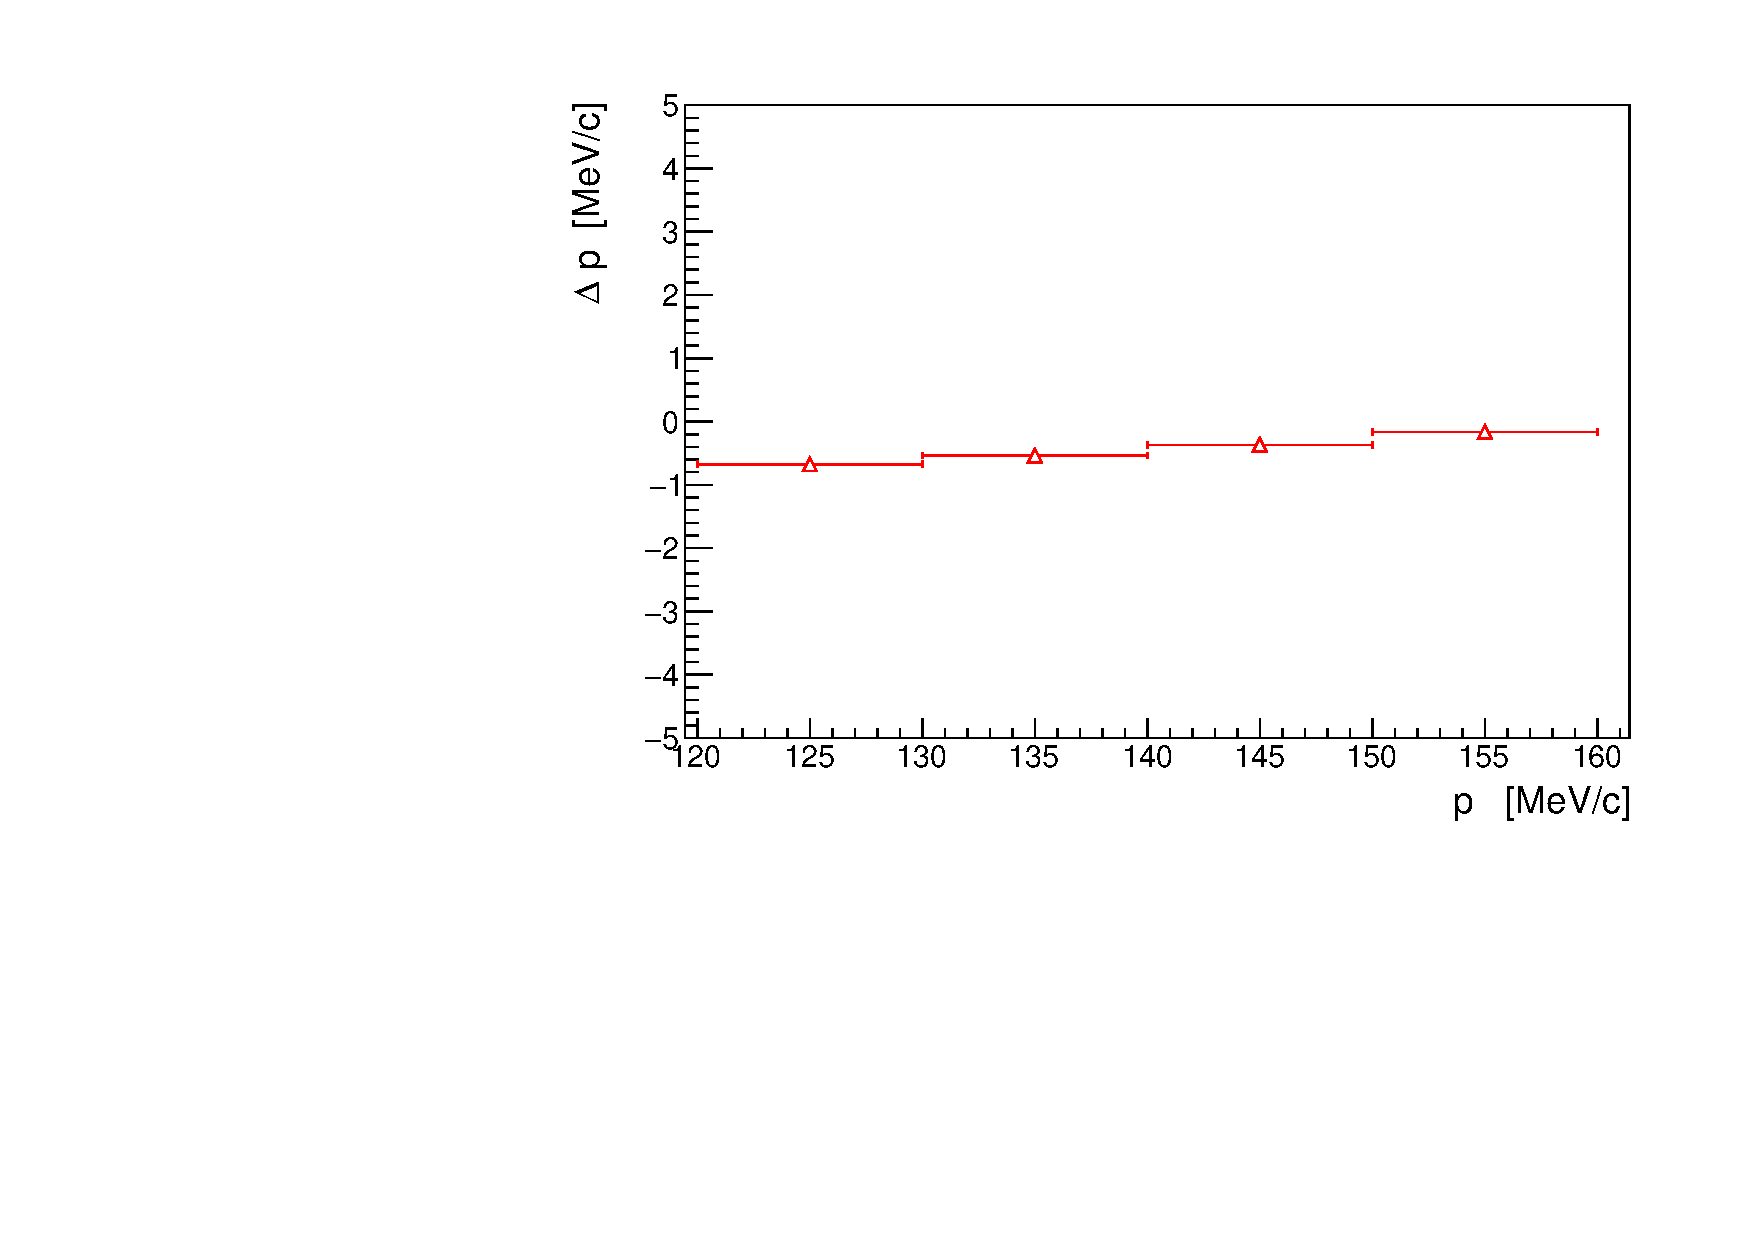
\includegraphics[width=0.5\textwidth]{upstream_p_bias_p.pdf} &	
        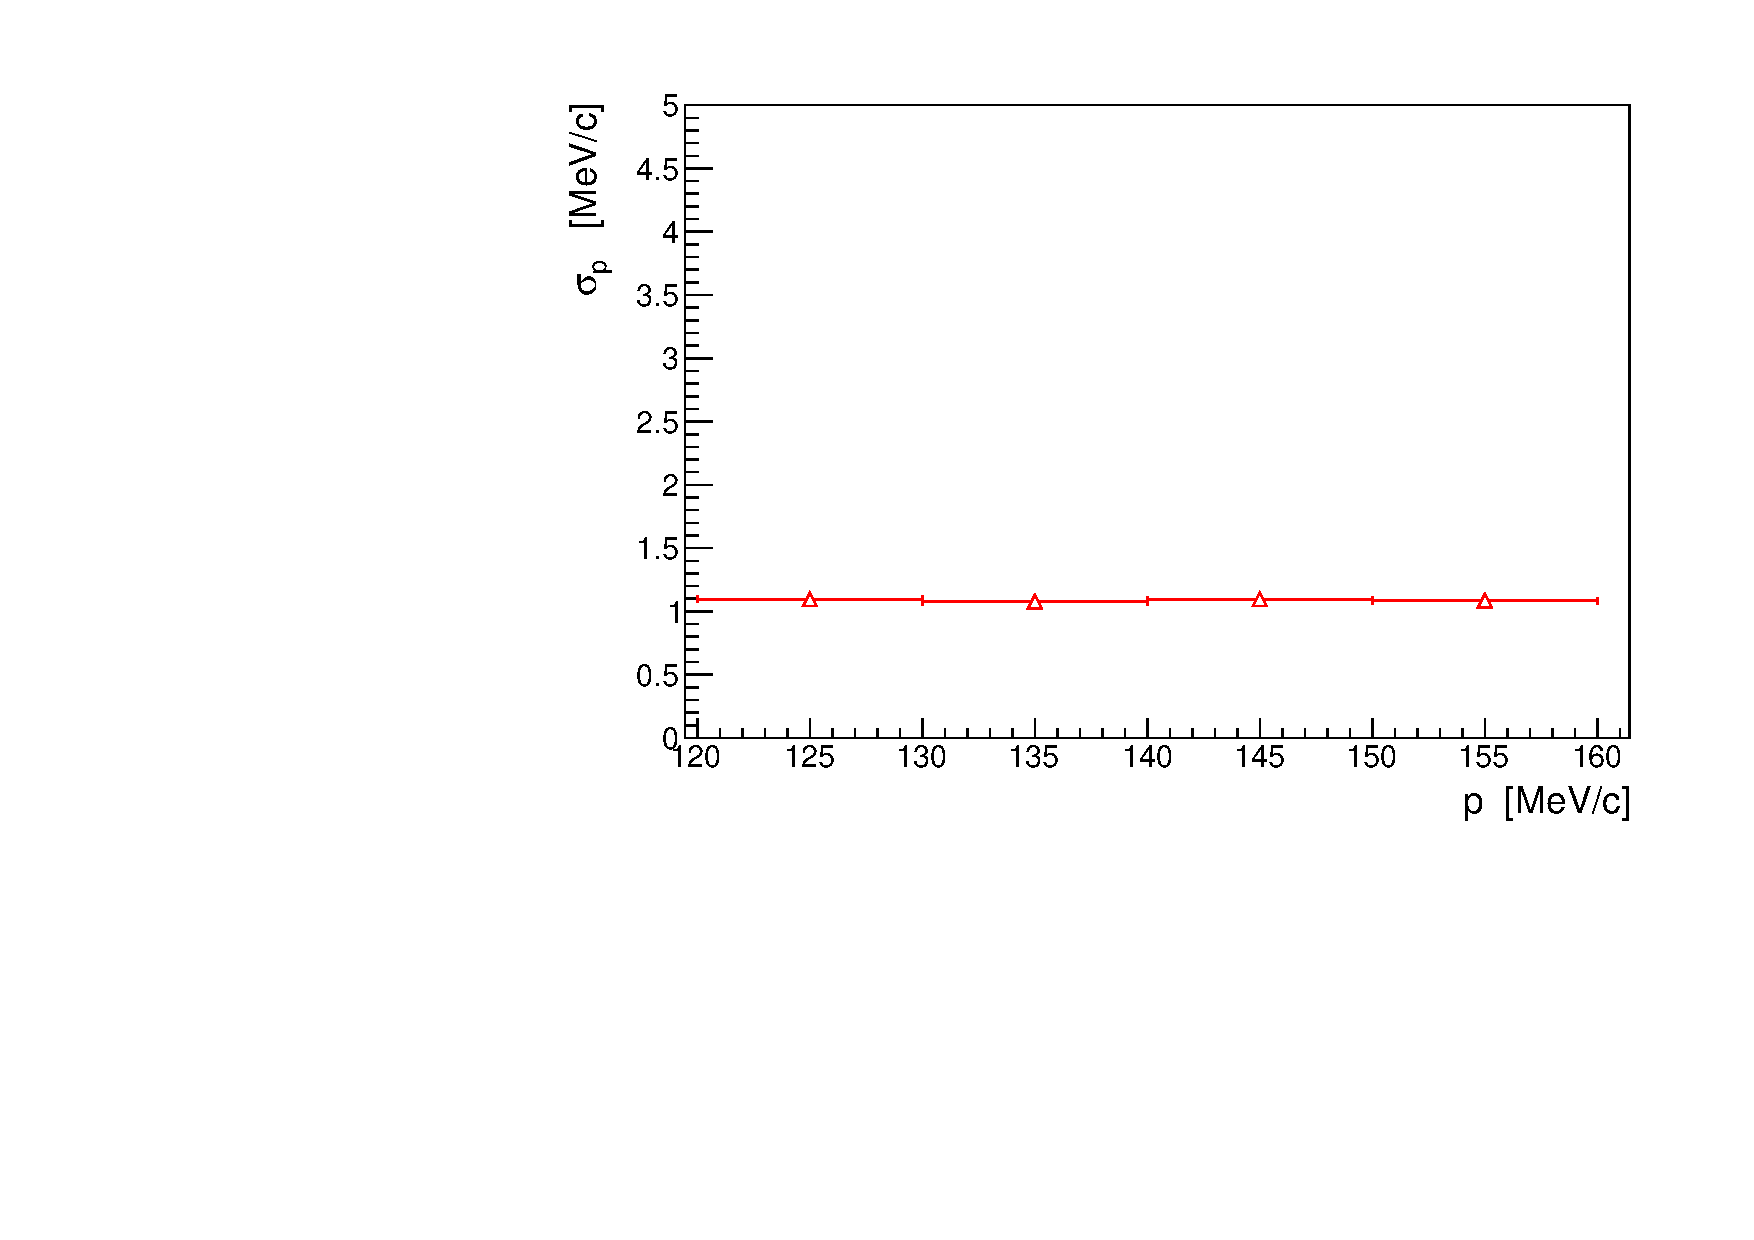
\includegraphics[width=0.5\textwidth]{upstream_p_resolution_p.pdf} \\
        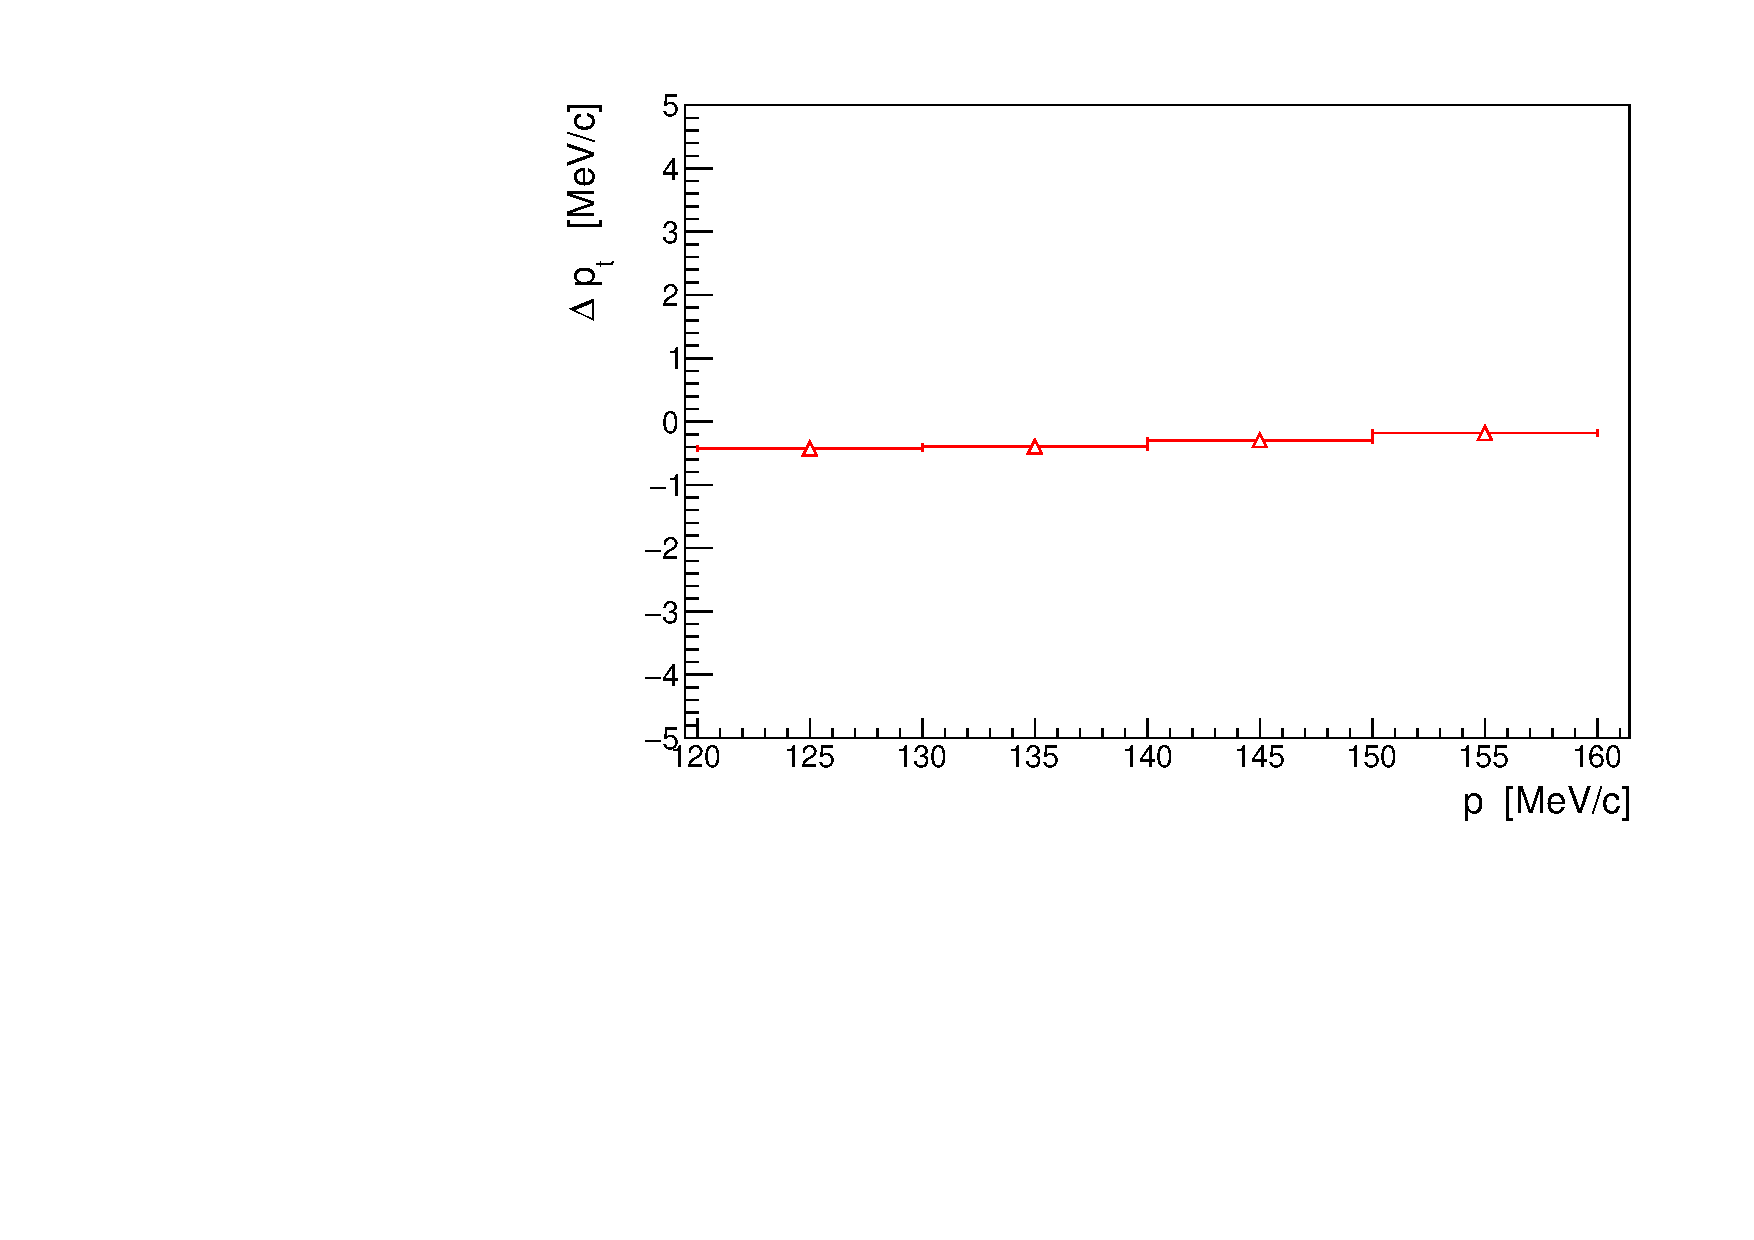
\includegraphics[width=0.5\textwidth]{upstream_pt_bias_p.pdf} &
        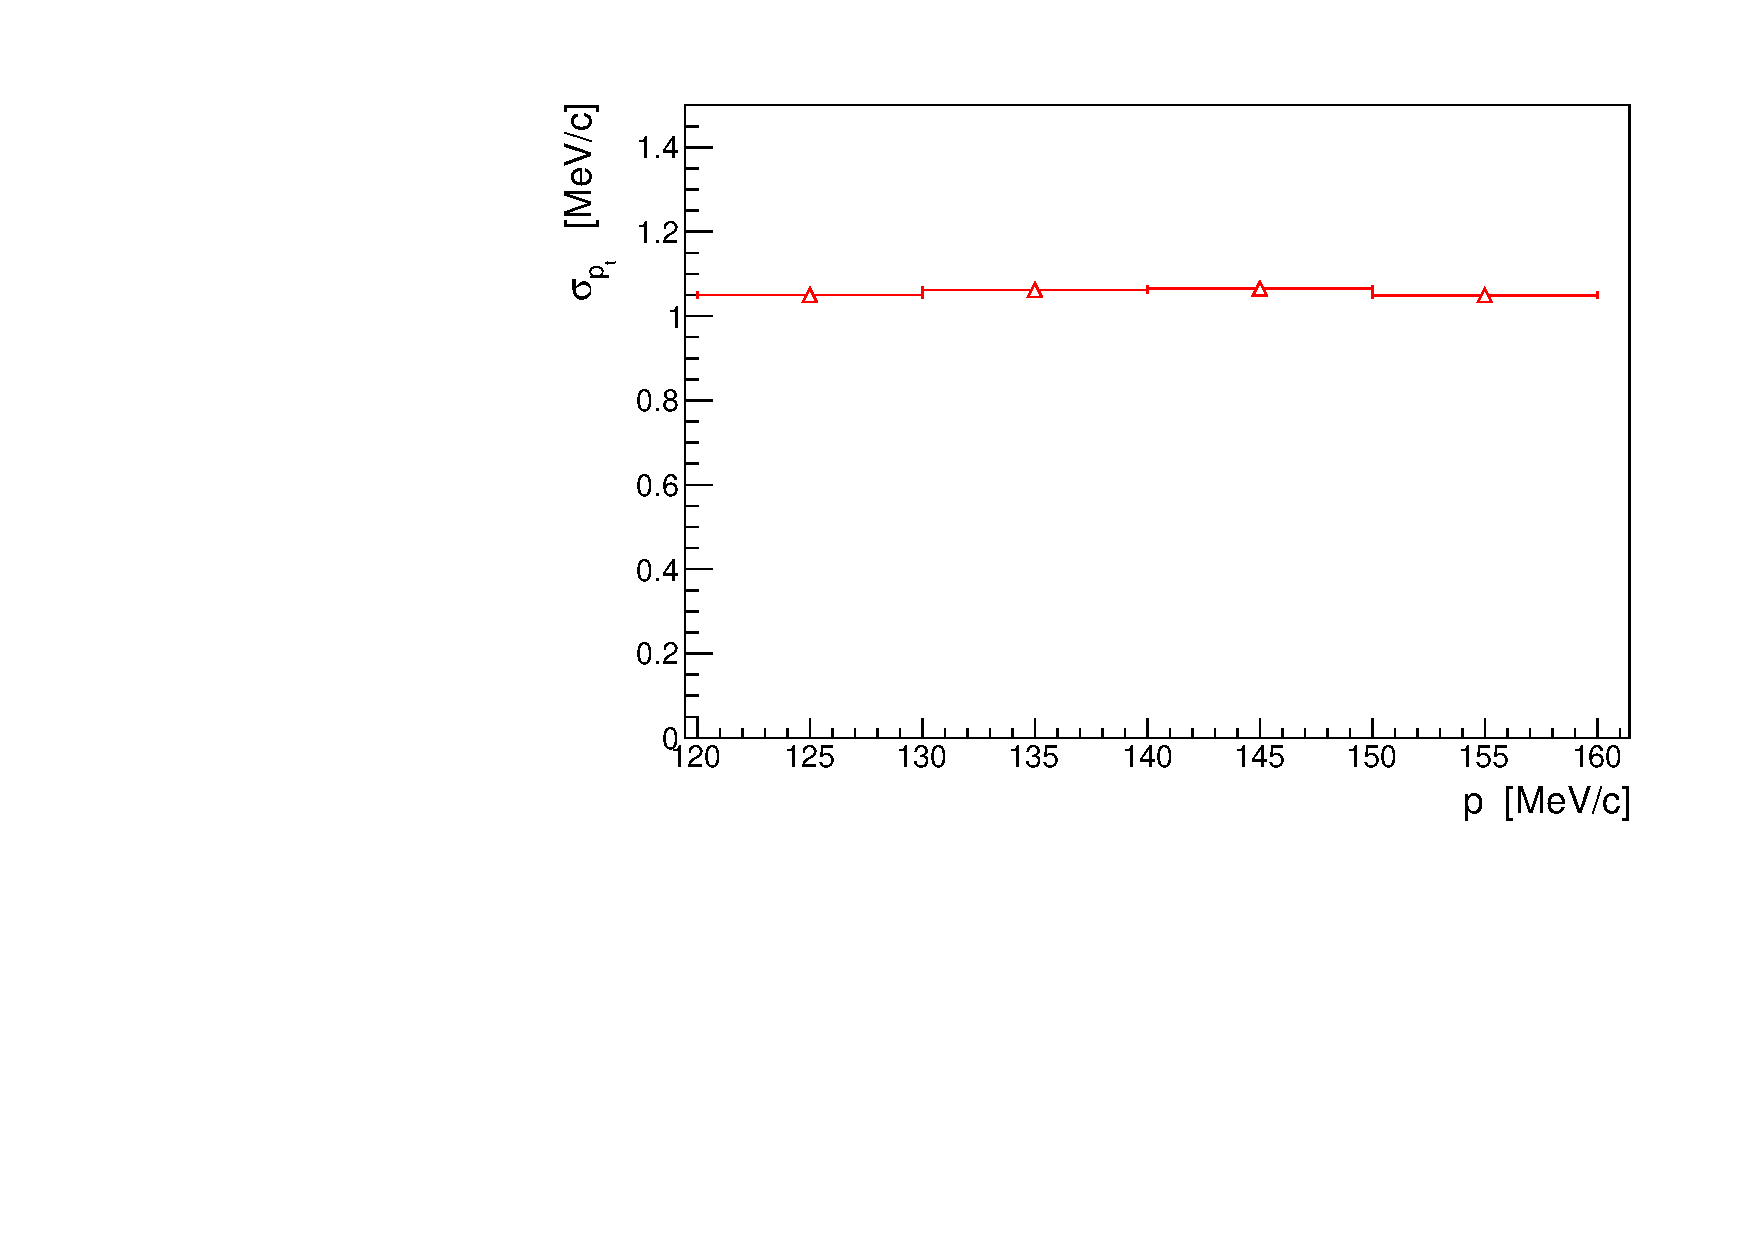
\includegraphics[width=0.5\textwidth]{upstream_pt_resolution_p.pdf}
    \end{tabular}
	\caption{\label{trackers:performance:resolutions:up}Predicted momentum reconstruction bias (left) and resolution (right) for the longitudinal (top) and transverse (bottom) momentum components in the upstream tracker.}
\end{figure}

\begin{figure}[ht]
	\centering
    \begin{tabular}{cc}
	    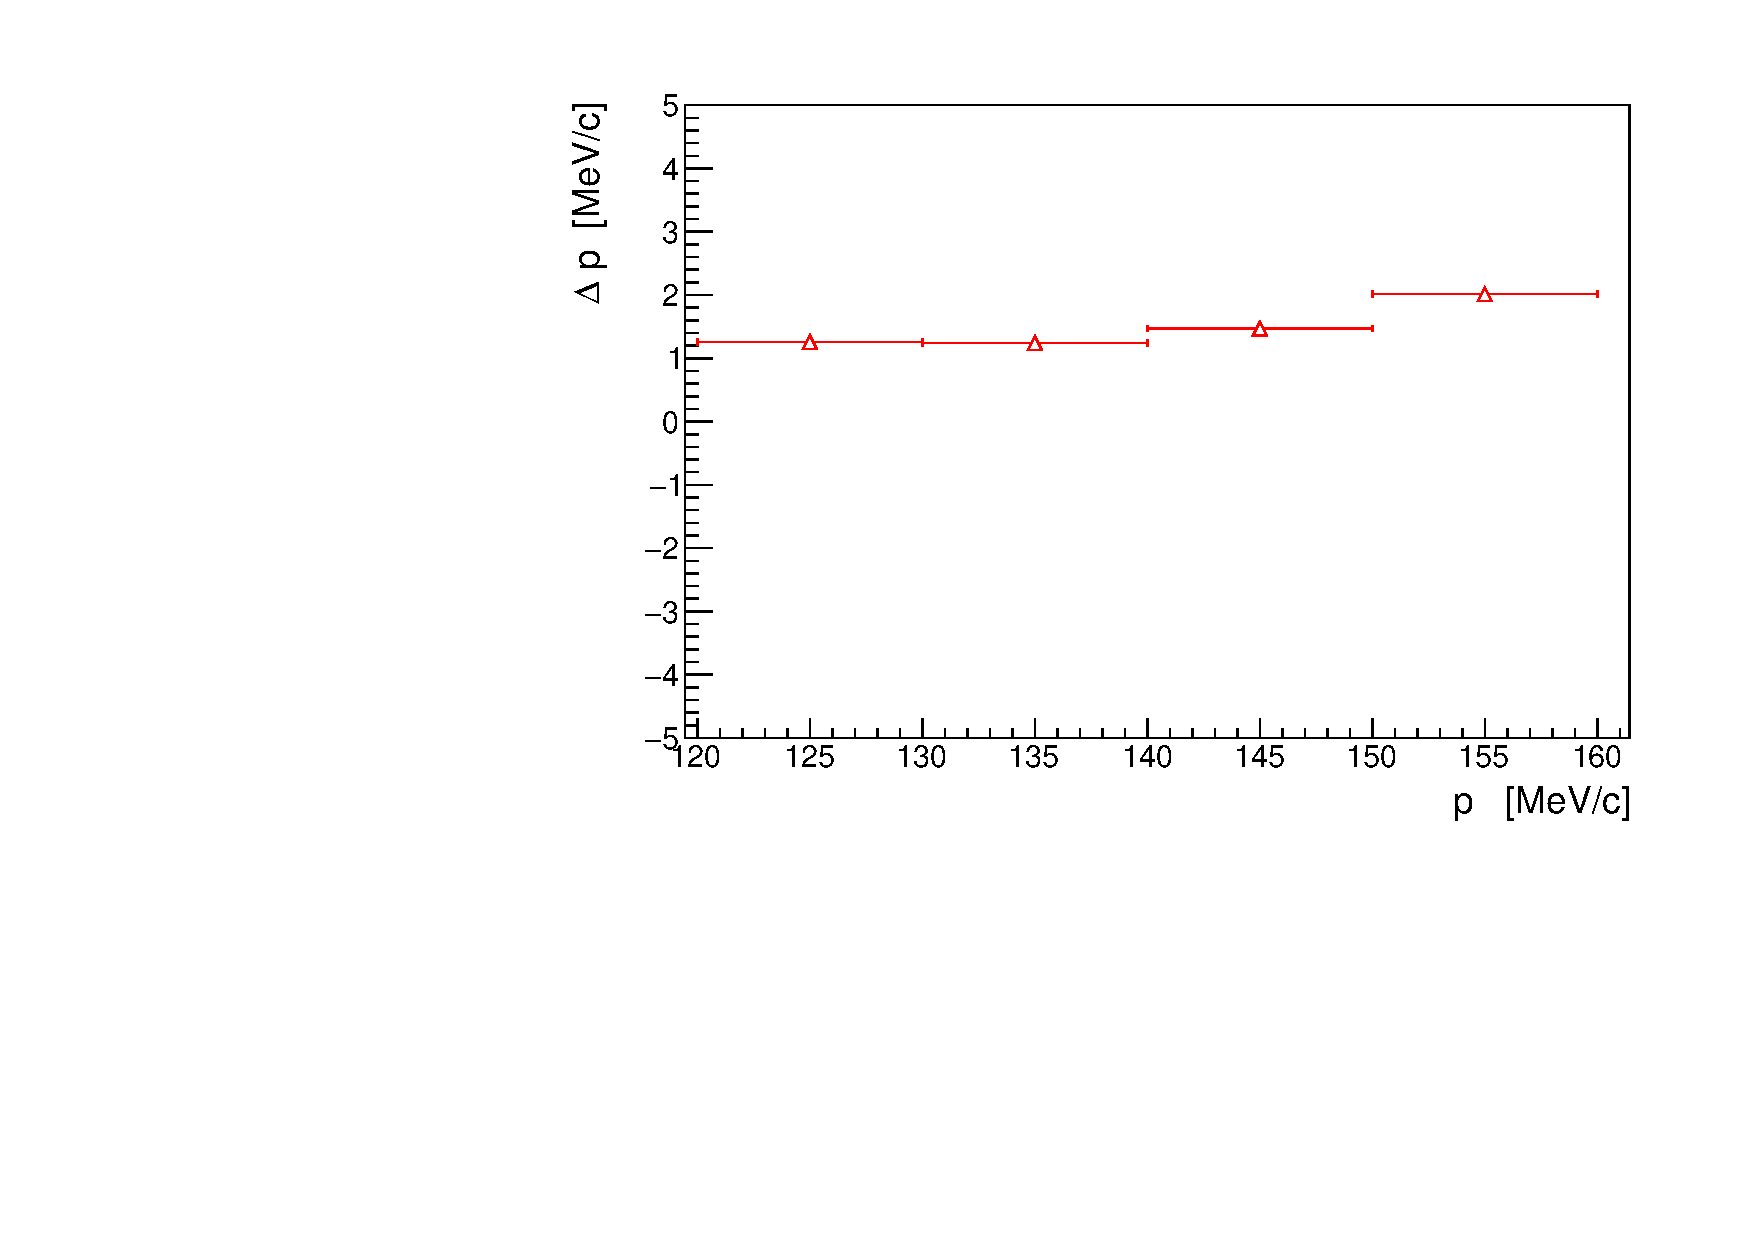
\includegraphics[width=0.5\textwidth]{downstream_p_bias_p.pdf} &	
        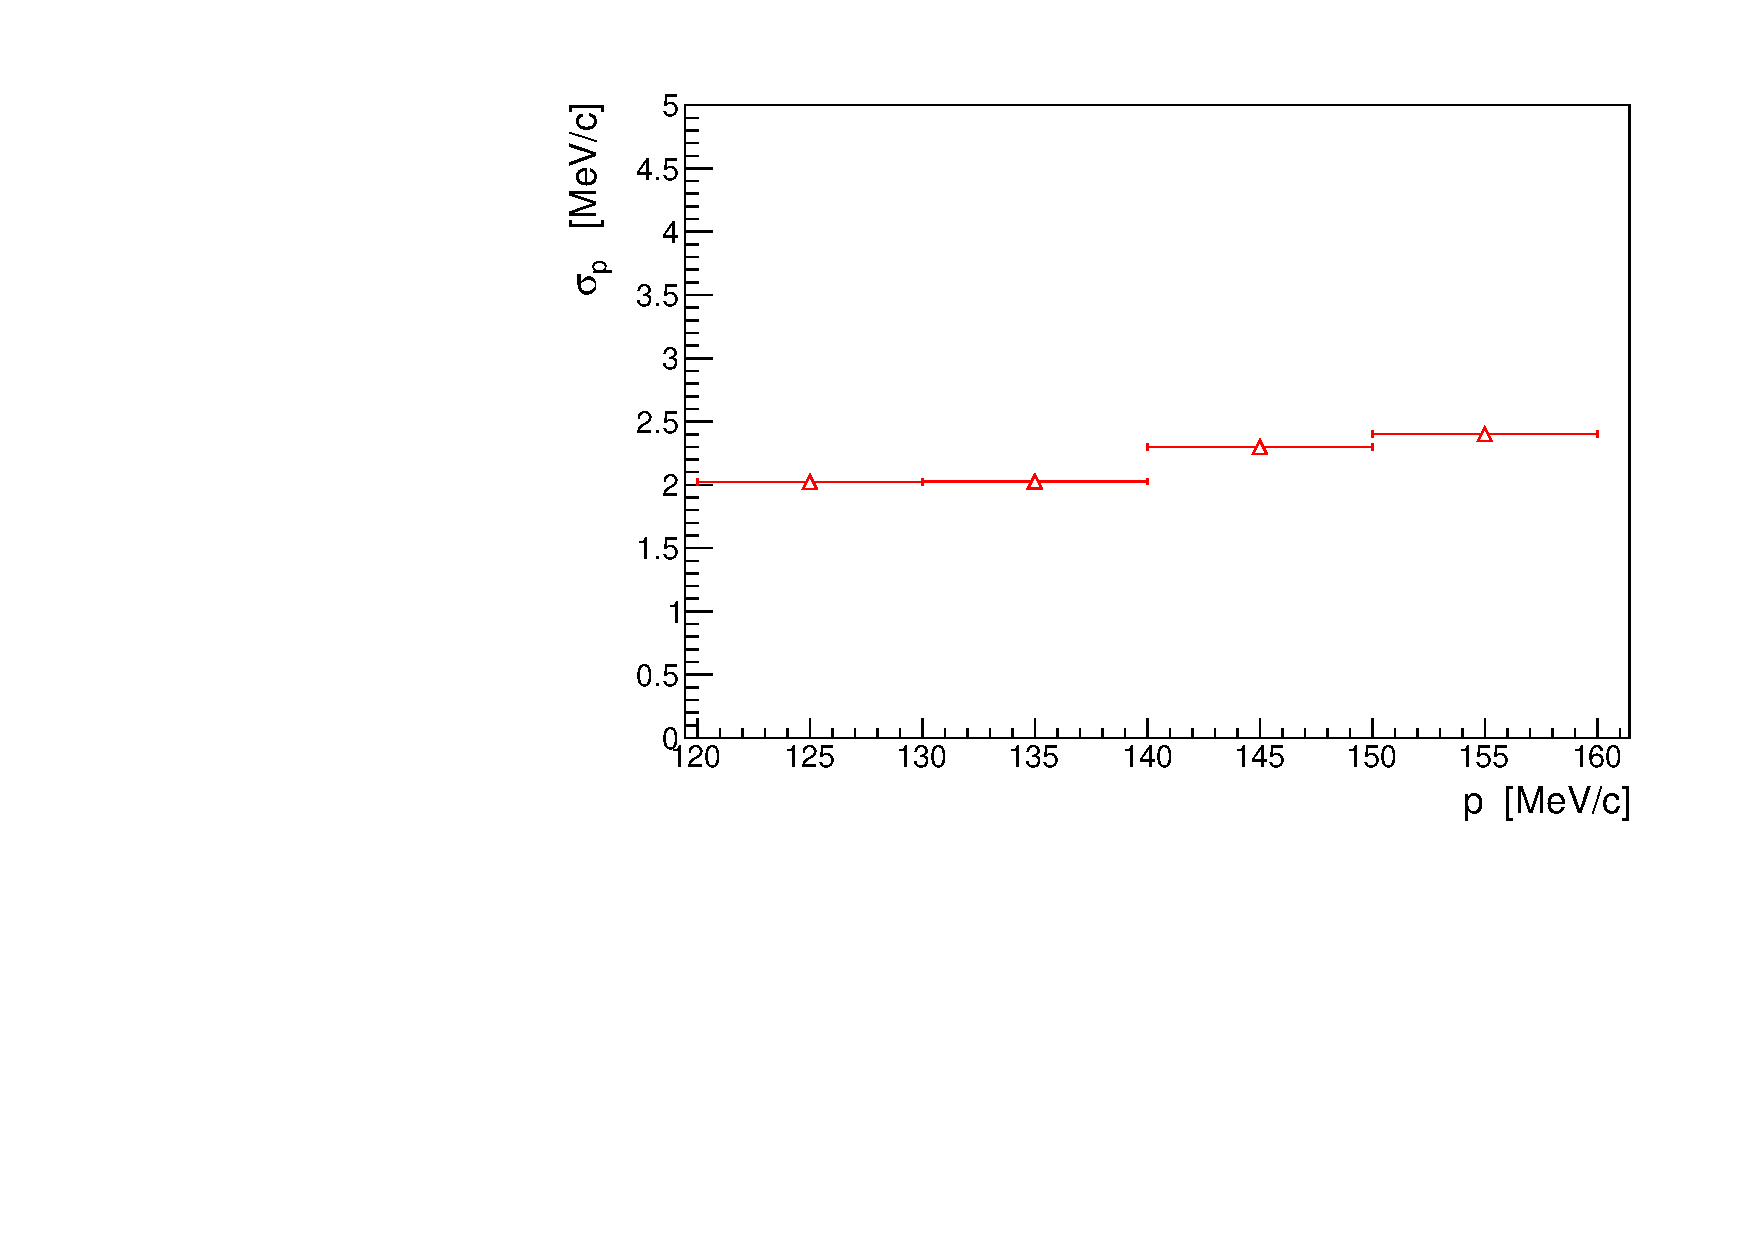
\includegraphics[width=0.5\textwidth]{downstream_p_resolution_p.pdf} \\
        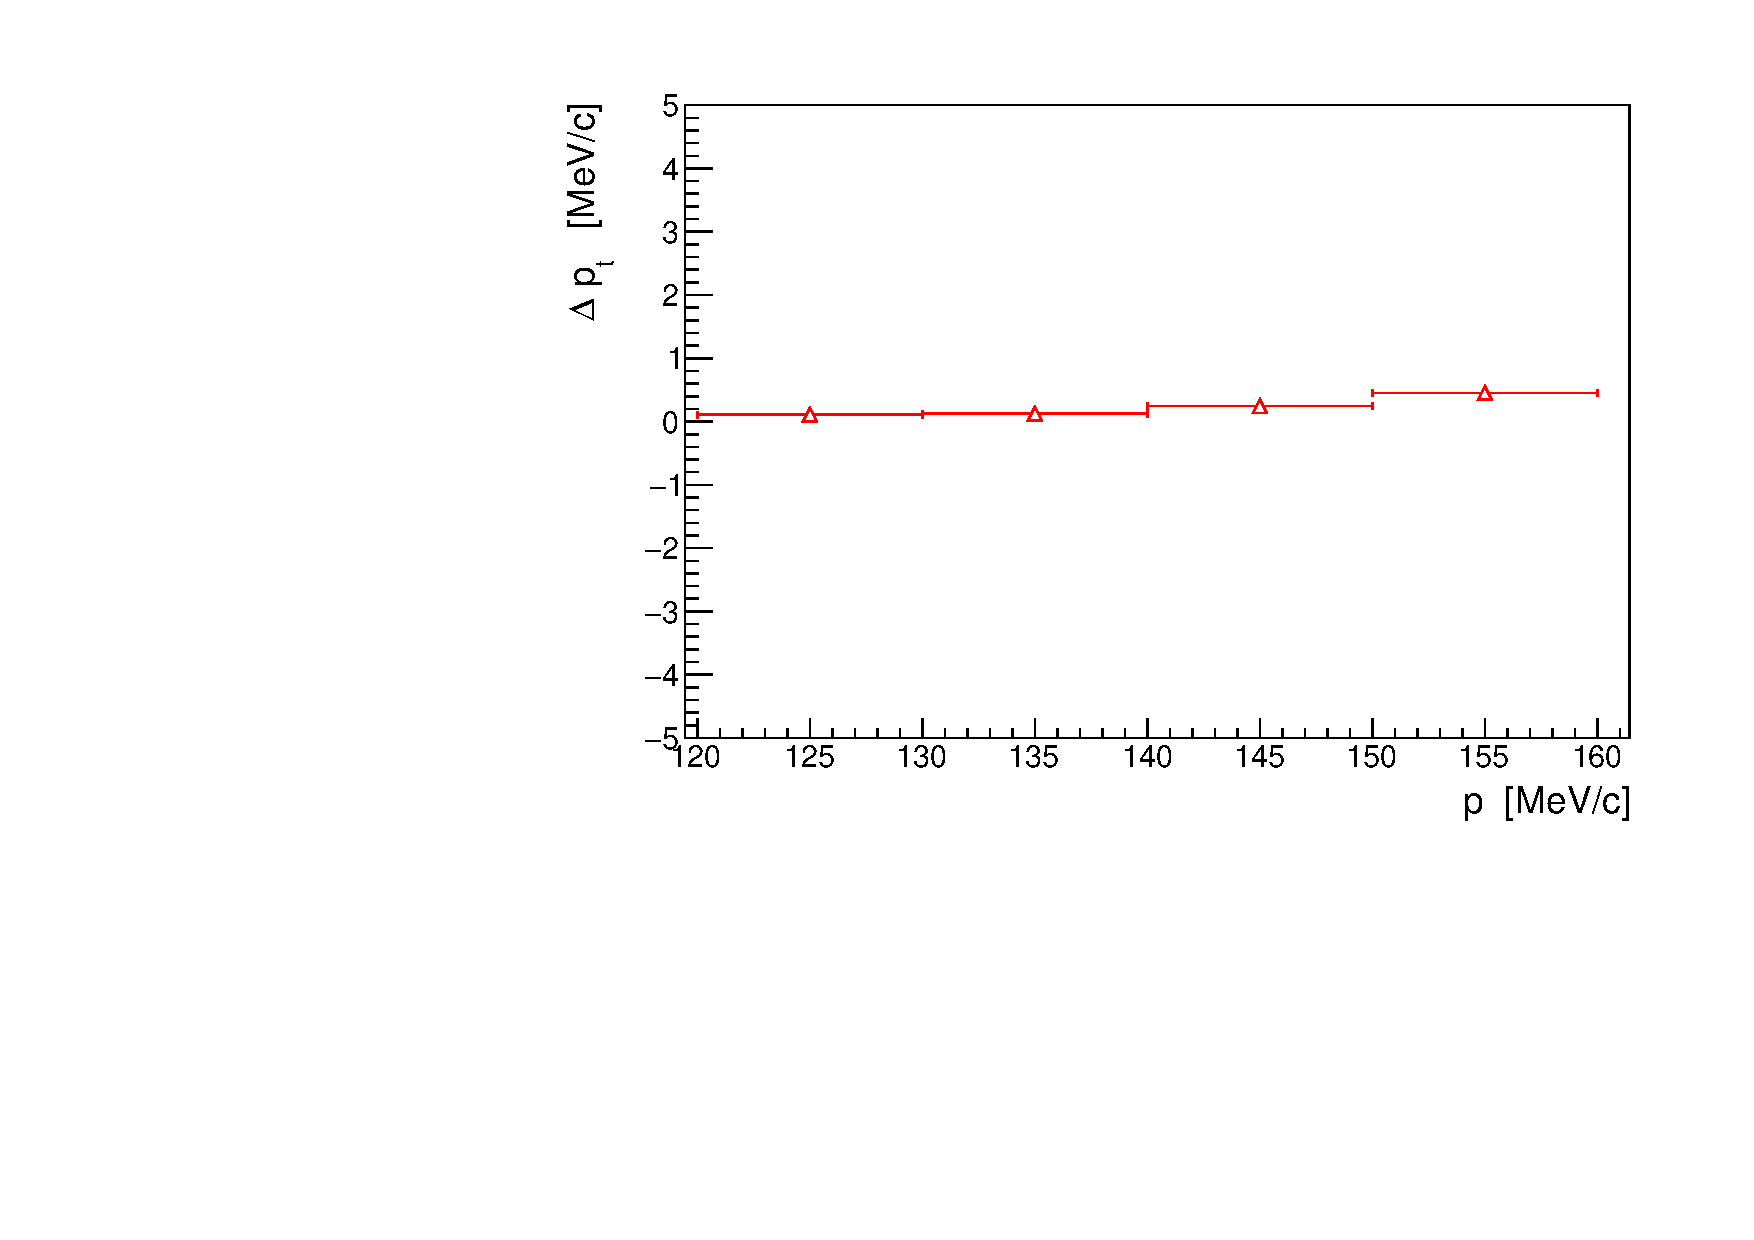
\includegraphics[width=0.5\textwidth]{downstream_pt_bias_p.pdf} &
        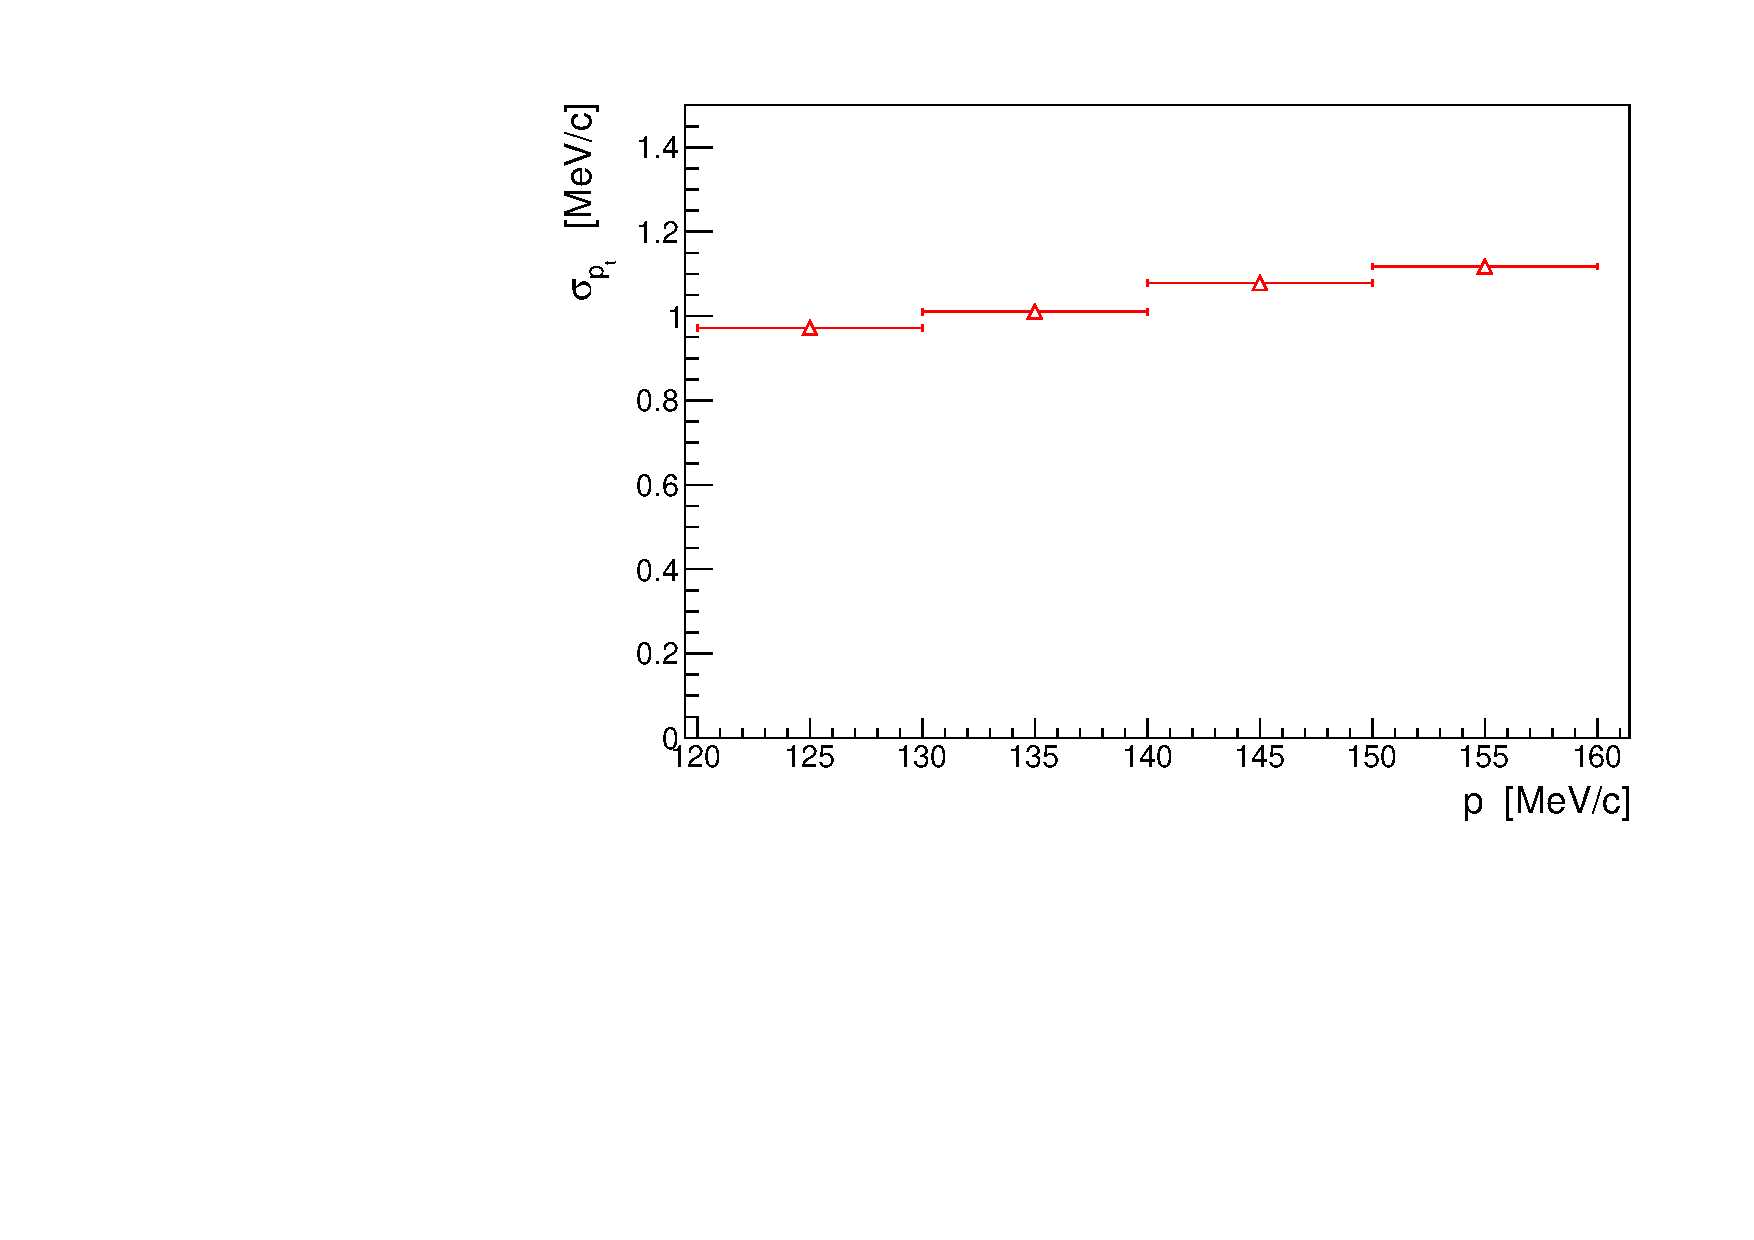
\includegraphics[width=0.5\textwidth]{downstream_pt_resolution_p.pdf}
    \end{tabular}
	\caption{\label{trackers:performance:resolutions:down}Predicted momentum reconstruction bias (left) and resolution (right) for the longitudinal (top) and transverse (bottom) momentum components in the downstream tracker.}
\end{figure}


\subsection{Efficiency evolution}

The efficiency of the tracker was processed over the lifetime of its use during the data taking. The analysis used in section~\ref{trackers:performance:efficiency} was repeated and automated for runs starting in 2015. The evolution of the helical track finding efficiency in the upstream and downstream trackers is shown in Fig.~\ref{fig:trackers:performance:historical}.

\begin{figure}
  \centering
  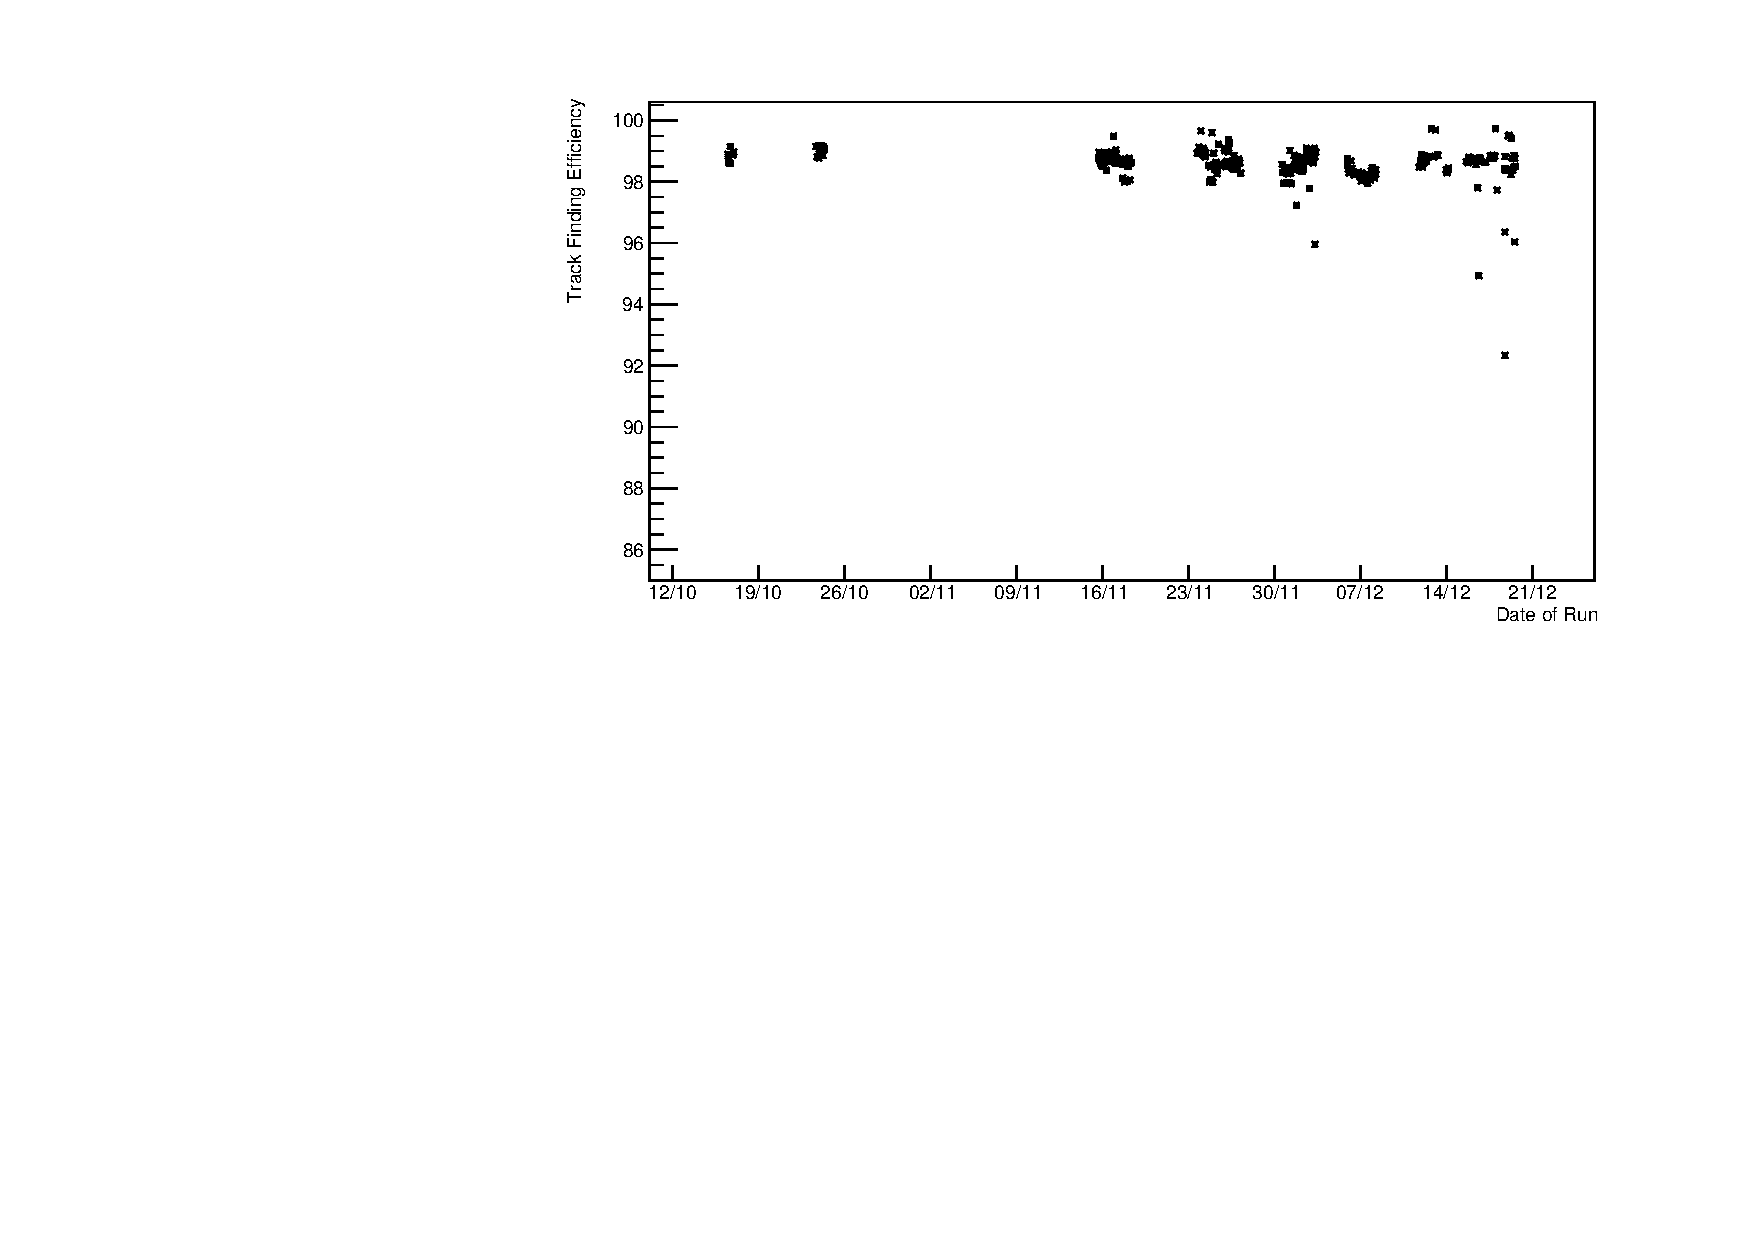
\includegraphics[width=0.8\textwidth]{upstream_historical_efficiency__helical.pdf}
  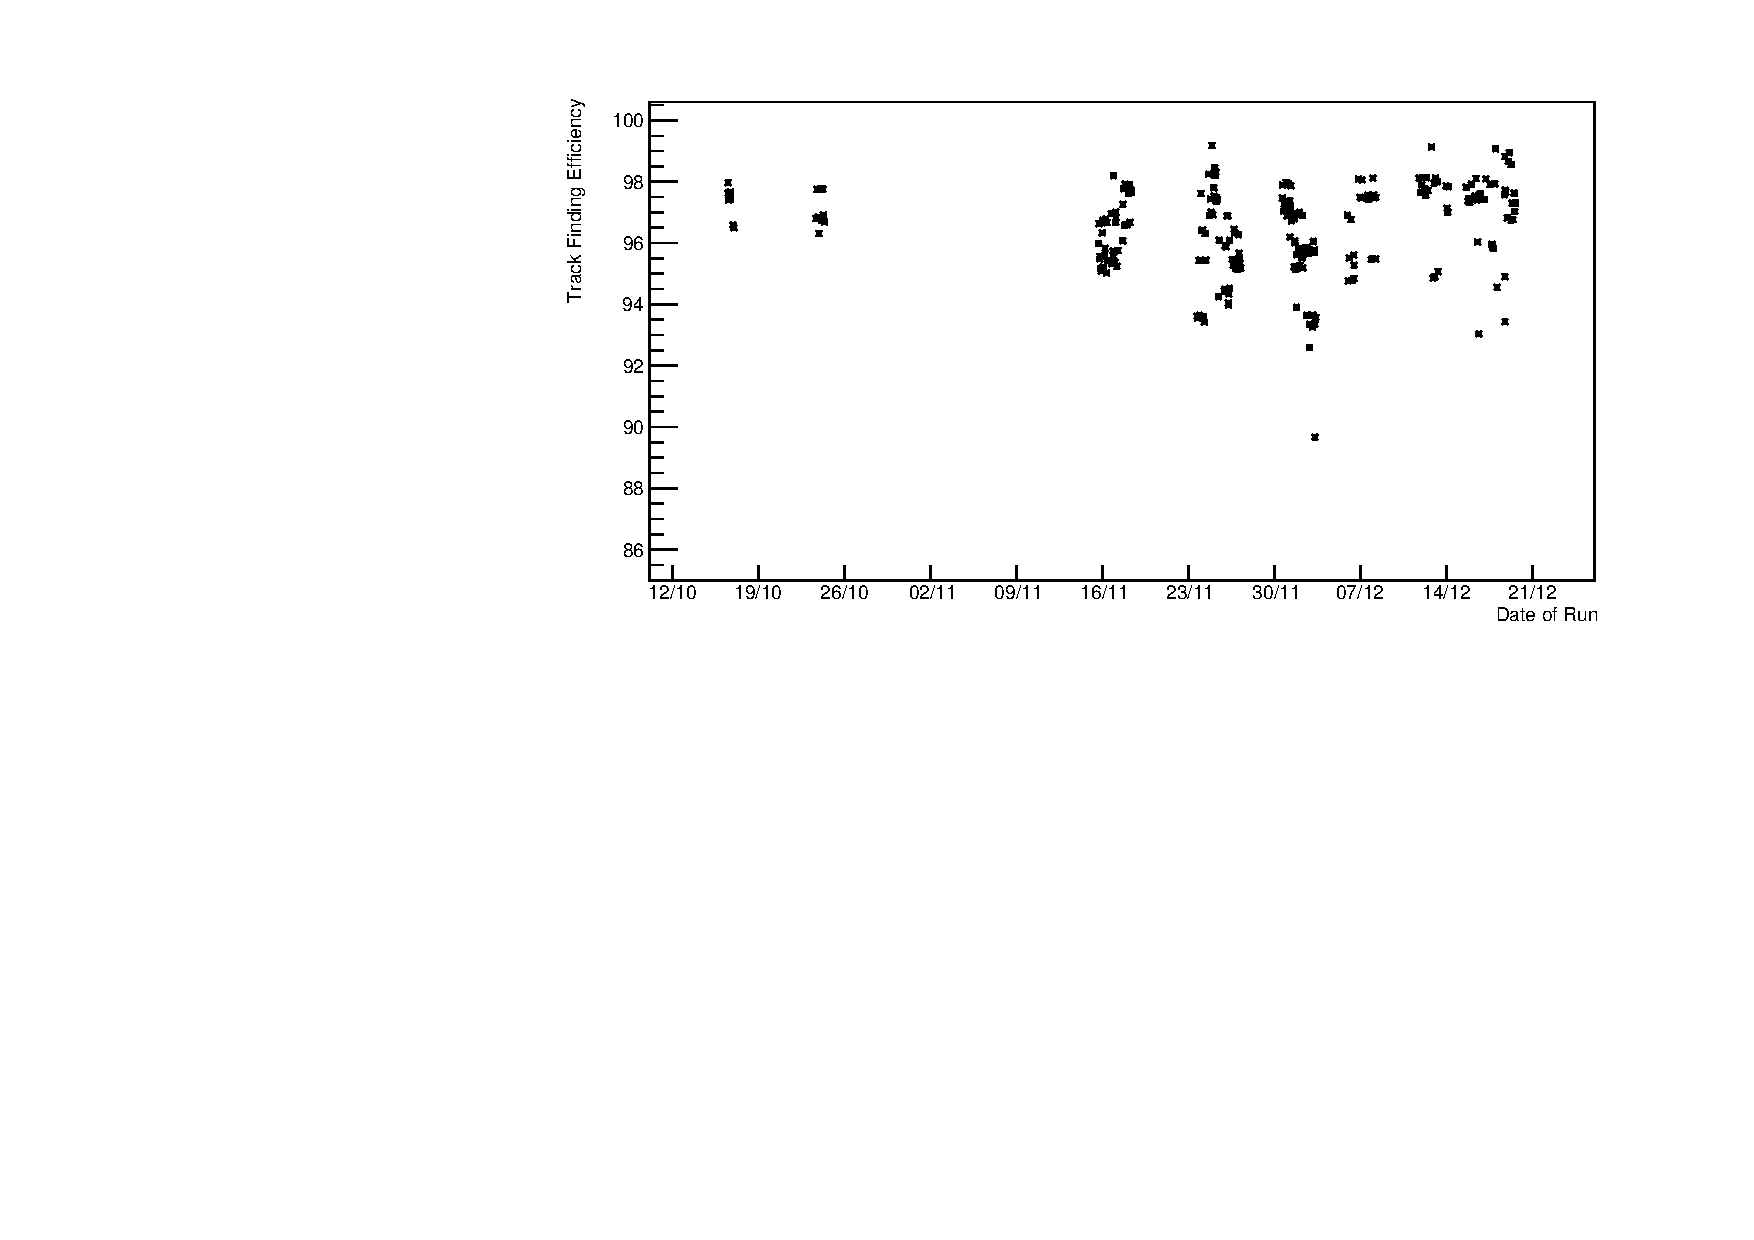
\includegraphics[width=0.8\textwidth]{downstream_historical_efficiency__helical.pdf}
  \caption{\label{fig:trackers:performance:historical}Evolution of the helical track finding efficiency over time for the upstream (top) and downstream (bottom) trackers during the key periods of data taking in 2016.}
\end{figure}
